\part{Container deployment and orchestration}
	\chapter{Productieomgeving}
	Een applicatie kan over een groot aantal services beschikken, die allemaal gebruik maken van verschillende technologiën. Een service kan eigenlijk beschouwd worden als een kleine applicatie, zodat er in plaats van één grote applicatie, meerdere kleinere applicaties in productie moeten draaien. Zo een productieomgeving moet vier functionaliteiten implementeren:
	\begin{enumerate}
		\item \textbf{Service management interface:} Het in staat zijn om services te creëren, configureren en updaten, vaak via een shell of GUI.
		\item \textbf{Runtime service management:} De omgeving moet automatisch services kunnen herstarten indien deze gecrasht zijn. Ook als een fysieke server faalt, moet de omgeving een andere server aanspreken om de service op te draaien.
		\item \textbf{Monitoring:} Informatie over elke service instance zoals logbestanden en metrieken voor die bepaalde service (aantal bezoekers per seconde, success rate, ...) moeten beschikbaar zijn voor de ontwikkelaars, en moeten ook gewaarschuwd worden indien een service niet aan de vooropgestelde criteria voldoet.  
		\item \textbf{Request routing:} De requests dat users versturen moeten naar de juiste service doorverwezen worden.
	\end{enumerate}
	Volgende paragrafen bespreken hoe een aantal van deze zaken geïmplementeerd kunnen worden.

	Een service heeft altijd een aantal configuratiegegevens (\textbf{environment variabelen} genoemd), die afhankelijk zijn van de omgeving waarin de service draait. Een service moet zo ontworpen zijn dat deze slechts éénmaal gecompileerd moet worden door de deployment pipeline, waarna deze meerdere malen in productie kan gezet worden. Het externaliseren van de configuratiegegevens betekent dat de configuratie van een service tijdens runtime bepaalt wordt. Hier zijn er twee modellen mogelijk:
	\begin{itemize}
		\item \textbf{Push model:} Bij dit model zal de service bij het opstarten configuratiegegevens verwachten, die door de deploymentomgeving meegegeven worden. Hoe deze configuratiegegevens gegeven worden (via bestand, of individuele parameters) maakt niet uit. De service en deploymentomgeving moeten wel onderling van elkaar weten hoe de structuur van de configuratiegegevens in elkaar zit. Het \underline{grootste nadeel} van deze methode is dat een service haast niet meer gewijzigd kan worden na het initialiseren van de service. Een ander \underline{nadeel} is dat de configuratiegegevens verspreidt over de services liggen.
		\item \textbf{Pull model:} Het pull model heeft bijna enkel voordelen tegenover het push model. De deploymentomgeving geeft bij de creatie van de service enkel de URL mee van een zogenaamde \underline{configuratieserver}. Deze server bevat alle configuratiegegevens voor elke service. De service zelf zal dan deze server, met behulp van de URL, aanspreken om de juiste configuratiegegevens op te halen. Dit biedt een aantal \underline{voordelen}:
		\begin{itemize}
			\item Gecentraliseerde configuratie.
			\item Een service kan de server pollen om na te gaan of de configuratiegegevens aangepast zijn, en deze dan eventueel op te halen. De service moet hiervoor niet herstart worden.
			\item Sommige configuratiegegevens zijn gevoelig, zoals database informatie. De server zal deze moeten encrypteren. De service wordt dan wel verwacht de publieke sleutel van de server te hebben zodat hij deze kan decrypteren. Sommige servers decrypteren de configuratiegegevens zelf.
		\end{itemize}
		Het \underline{grootste nadeel} is echter dat de configuratieserver opnieuw een infrastructuur is dat moet opgesteld en onderhouden worden.
	\end{itemize}

	Om \textbf{monitoring} te implementeren moeten services 'waarneembaar' gemaakt worden. Er moeten hiervoor extra APIs aangemaakt worden, die niet mogen interfereren met de werkelijke functionaliteit van de service. Hiervoor zijn er een aantal hulpmiddelen om een service waarneembaar te maken:
	\begin{itemize}
		\item \textbf{Health check API.} Een eenvoudige API dat de status van de service teruggeeft.
		\item \textbf{Log aggregation.} Logbestanden zijn een goede manier om de werking van de service op te volgen. Deze logbestanden worden best geschreven naar een gecentraliseerde logserver, zodat \underline{zoeken} ondersteund kan worden. Het is ook enkel de verantwoordelijkheid van de logserver om ontwikkelaars te waarschuwen. Traditioneel logt een applicatie naar een welbepaald logbestand op het filesysteem. Dit is hier geen goede oplossing, omdat sommige services zelfs geen filesysteem zullen hebben. Hierom moet elke service loggen naar stdout. De deploymentomgeving zal dan beslissen wat hij wil doen met deze uitvoer. 
		\item \textbf{Distributed tracing.} Het oproepen van een endpoint van de API kan meerdere interne calls maken. Het is vaak moeilijk te achterhalen waarom een query traag verloopt. Distributed tracing kent aan elke endpoint een ID toe, en bekijkt de call chain die overlopen wordt. Deze gegevens worden naar een gecentraliseerde server verstuurd waarop analyse kan uitgevoerd worden. Een endpoint wordt gepresenteerd door een \underline{trace}. Zo een trace bestaat uit geneste \underline{spans}, die elk een call voorstellen. De endpoint is de top span, en zal elke andere span bevatten. 
		\item \textbf{Audit logging.} Het doel van audit logging is om acties van gebruikers te verzamelen. Elke audit log entry heeft een ID dat een gebruiker voorstelt, de actie dat ze uitgevoerd hebben en het domeinobject waarop de actie uitgevoerd wordt. Voorbeelden zijn gefaalde loginpoging of toevoegen van items in het winkelmandje, maar uiteindelijk niet betalen. Zulke logs dienen vooral voor customer support en om vreemde activiteiten op te sporen.
		\item \textbf{Application metrics.} Deze tak bestaat uit een metriekservice. Deze metriekservice vraagt gegevens op van de verschillende applicaties. Zulke gegevens zijn onder andere: processorgebruik, geheugengebruik, schijfgebruik, aantal requests per seconde, request latency en domeinspecifieke gegevens. Een service moet ontworpen zijn zodat al deze gegevens naar de metriekservice kunnen verstuurd worden, en is afhankelijk van het gebruikte framework. De service kan ofwel zelf beslissen om zijn metrieken te versturen naar de metriekservice, of de metriekservice zal elke service pollen om de metrieken op te halen.
	\end{itemize}
	\chapter{Containers}
	Verschillende microservices kunnen onderling elk gebruik maken van verschillende technologiën. Om deze verschillende microservices te deployen zouden al de verschillende dependencies van elke technologie op de server geconfigureerd moeten worden. Dit is natuurlijk niet haalbaar op grote schaal, daarom zou men in eerste instantie virtuele machines kunnen gebruiken waarbij elke verschillende virtuele machine geschikt is voor een specifieke technologiestack. Virtuele machines nemen echter te veel opslag in beslag. Ze nemen zoveel beslag in omdat elke virtuele machine zijn eigen besturingssysteem en kernel bevat. De hypervisor (of virtual machine monitor) geeft elke virtuele machine de illusie dat enkel hun machine toegang heeft tot de resources van het \underline{hosttoestel} (het toestel waarop de virtuele machines draaien). 
	Er zijn twee types hypervisor:
	\begin{itemize}
		\item \textbf{Type 1.} Dit type hypervisor draait rechtstreeks op de hardware van de host en heeft geen behoefte aan een onderliggend besturingssysteem. 
		\item \textbf{Type 2.} Dit type hypervisor heeft wel nood aan een besturingssysteem. Dit heeft als voordeel dat er ook applicaties op het hosttoestel kunnen draaien.
	\end{itemize}
	\underline{Containers} zijn een virtualisatietechniek op besturingssysteemniveau. Een populaire container technologie is Docker, dat gebruik maakt van de linux container functionaliteit. Docker maakt gebruik van \uline{vier linux concepten:}
	\begin{itemize}
		\item \textbf{Linux Control Groups (cgroups).} Groeperen van processen, en privileges zetten op deze groepen.
		\item \textbf{Linux namespaces.} Een geïsoleerde weergave van de systeemresources instellen voor cgroups.
		\item \textbf{Changing root (chroot).} Elk proces de illusie geven dat ze vanuit de root-directory aangesproken worden.
		\item \textbf{Veilige containers (LSM).} Mogelijkheden per proces vastzetten zoals access control.
	\end{itemize}

	\underline{Docker}:
	\begin{itemize}
		\item Automatisch verpakken en deployen van een applicatie.
		\item Beschikbaar op Linux, MacOS, Windows.
		\item Onafhankelijk. Minimale dependencies.
		\item Grote flexibiliteit in wat er in de container moet.
		\item Alle containers kunnen gestart en gestopt worden op dezelfde manier.
		\item Lightweight. Meerdere containers per host mogelijk (nog meer dan virtuele machines).
	\end{itemize}

	\section{Docker architectuur}
	\begin{figure}[ht]
		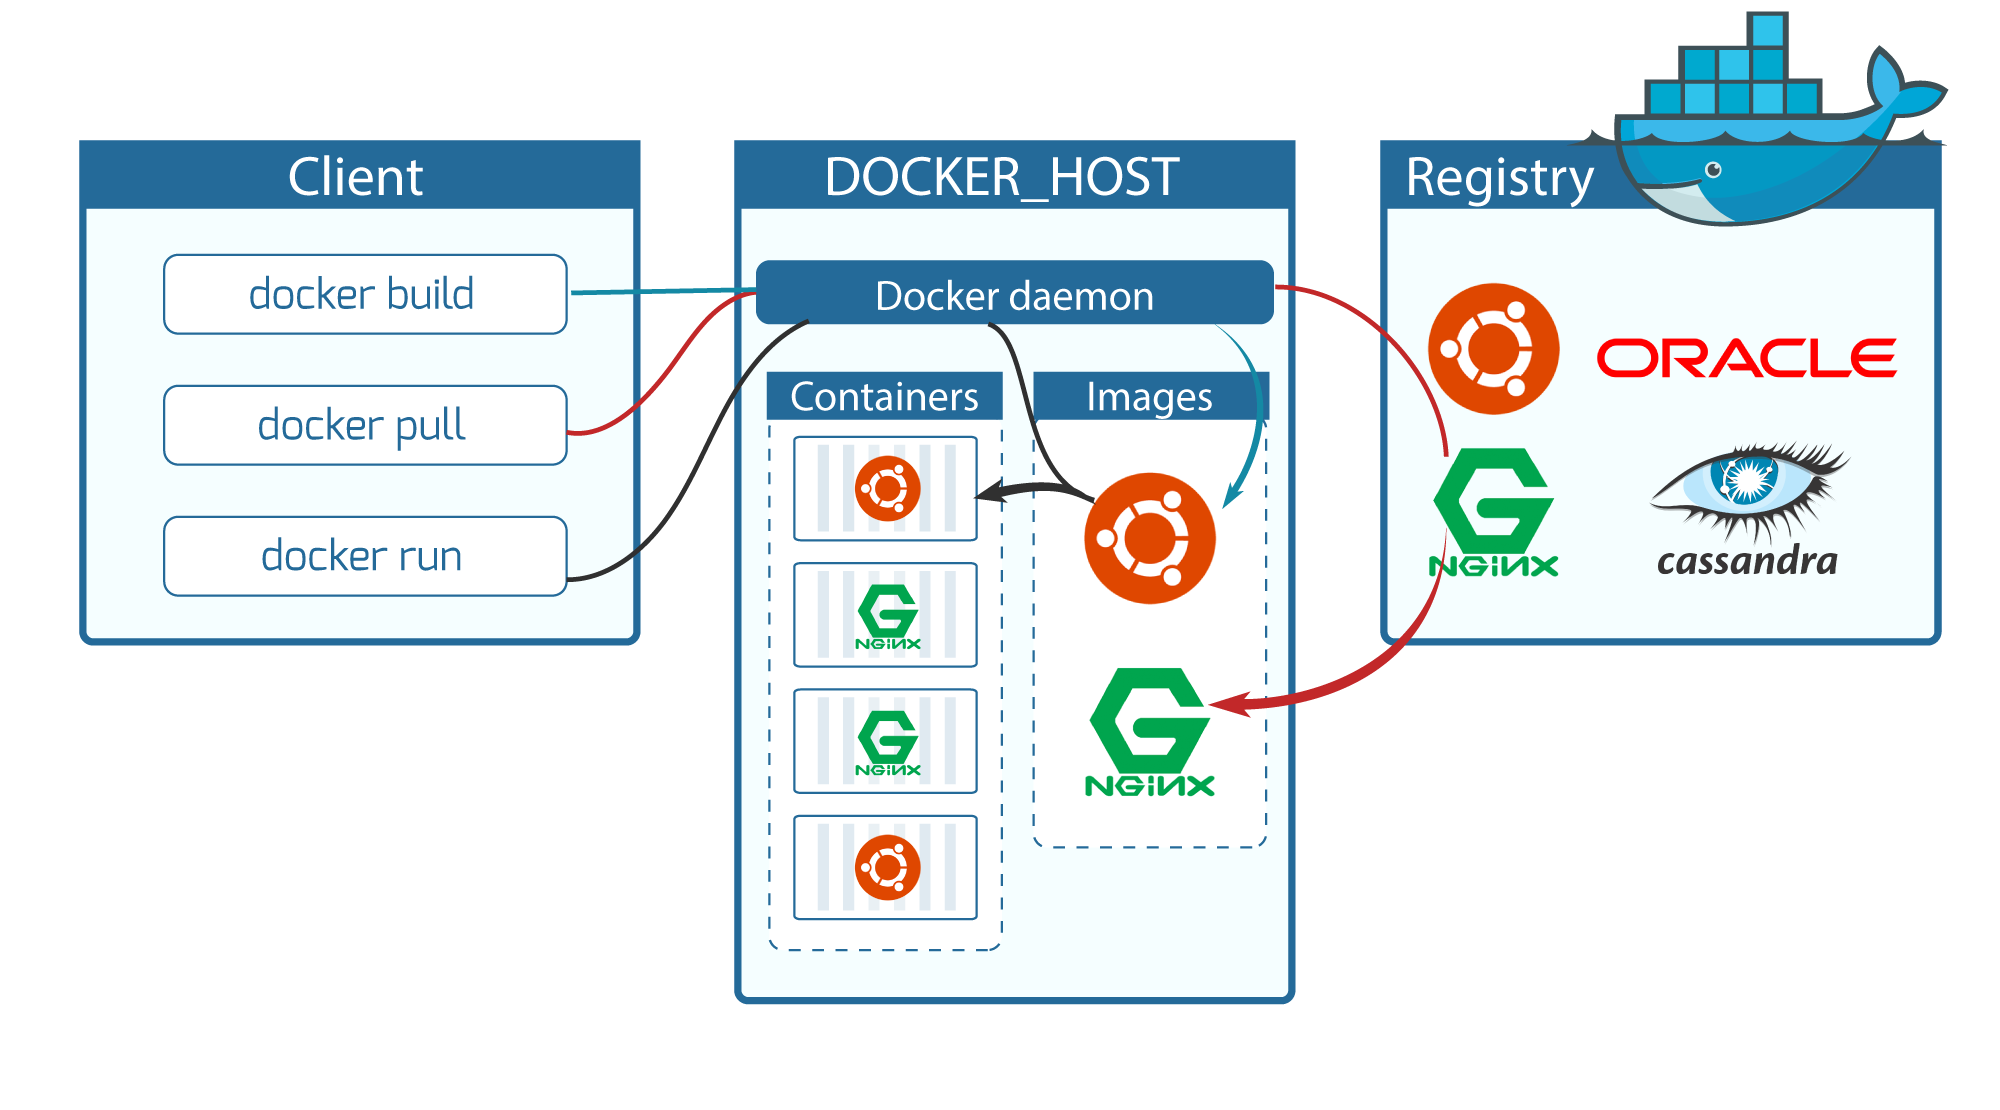
\includegraphics[width=\textwidth]{docker_architecture}
	\end{figure}
	De \textbf{Docker daemon} is verantwoordelijk om containers te starten, stoppen, monitoren, alsook om images op te slaan en te builden. De \textbf{Docker client} kan de daemon aanspreken om de operaties van de daemon uit te voeren. De \textbf{Registry} bevat images die door de daemon gebruikt kunnen worden.

	\underline{Een image aanmaken kan als volgt:}
	\begin{lstlisting}
# Dockerfile to build an Apache2 image
# Base image is Ubuntu
FROM ubuntu:14.04
# Install apache2 package
RUN apt-get update && apt-get install -y apache2 && apt-get clean
	\end{lstlisting}
	Uitvoeren van deze image zal ervoor zorgen dat containers met deze image kunnen gestart worden. Een image wordt gedeeld voor elke container en wordt telkens hergebruikt. Dit zorgt ervoor dat een container zelf weinig schijfruimte inneemt. Wanneer een container gestart wordt vanuit een image, dan zal Docker een extra schrijfbare laag toevoegen. Op deze laag kunnen dan nieuwe bestanden gezet worden. Als de container verwijderd wordt, zullen ook deze bestanden verwijderd worden. Op die manier kunnen verschillende containers, die toch dezelfde image hebben, aparte informatie bewaren. 

	\underline{Syntax van een Dockerfile}:
	\begin{lstlisting}[numbers=left]
FROM ubuntu:14.04

COPY html /var/www/html
ADD web-page-config.tar /

ENV APACHE_LOG_DIR /var/log/apache
USER 73

EXPOSE 7373/udp 8080

RUN apt-get update && apt-get install -y \ apache 2 && apt-get clean

ENTRYPOINT ["echo", "Dockerfile entrypoint Demo"]
	\end{lstlisting}
	\begin{itemize}
		\item  \textbf{Lijn 1 FROM} De base image van de container. Alle volgende commandos bouwen verder op deze image. 
		\item  \textbf{Lijn 3 COPY} Bestanden kopieren van de docker host naar het bestandssysteem van de nieuwe image.
		\item  \textbf{Lijn 4 ADD} Gelijkaardig aan COPY, maar kan ook .tar bestanden (die hij zal unzippen) en URLs (die hij zal downloaden) behandelen.
		\item  \textbf{Lijn 6 ENV} Een omgevingsvariabele instellen in de nieuwe image.
		\item  \textbf{Lijn 7 USER} Een gebruiker toevoegen met een specifiek UID. Deze UID wordt ook gebruikt in volgende RUN, CMD of ENTRYPOINT instructies.
		\item  \textbf{Lijn 9 EXPOSE} Deze instructie \underline{informeert} enkel dat  deze poorten zullen gebruikt worden. Docker zal zelf deze poorten niet openzetten.
		\item  \textbf{Lijn 11 RUN} Deze instructie bevat commando's die uitgevoerd moeten worden tijdens de buildfase. Het is beter om slechts één RUN instructie te hebben, omdat docker een nieuwe, read-only, laag aanmaakt voor elke instructie.
		\item  \textbf{Lijn 13 ENTRYPOINT} Het startpunt van de applicatie. Als deze applicatie stopt, wordt de container ook automatisch gestopt.
	\end{itemize}

	Verschillende containers die gebruik maken van dezelfde image kunnen toch bestanden van de image wijzigen. Docker maakt hier gebruik van een \underline{union filesysteem}. Zo een filesysteem neemt een bestaand filesysteem en mapt dit op een ander bestandssysteem. In het geval dat een bestand van een image gewijzigd moet worden, zal er eerst een kopie van de image naar de schrijfbare laag van de container gemaakt worden, waarna deze kopie aangepast wordt. 
	\chapter{Container orchestration}
	\underline{Drie functies van een orchestration framework}:
	\begin{enumerate}
		\item \textbf{Resource management}: Een groep van machines als één cluster beschouwen, zodat het lijkt alsof deze groep één proces is met zijn eigen CPU-, RAM- en volumegebruik.
		\item \textbf{Scheduling}: Bepalen welke groep van containers op welke machine moet komen. De default werkwijze is om te kijken naar de systeemresources die een groep nodig heeft, en een daarbij horende machine te vinden die deze systeemresources kan aanbieden.
		\item \textbf{Service management}: Het blootstelling van de container aan de externe wereld. Ook zal het framework ervoor zorgen dat er genoeg instanties van een bepaalde service zijn. Verder zal het framework load balancing implementeren tussen deze instanties.
	\end{enumerate}

	\section{Kubernetes}
	\underline{Kubernetes is een voorbeeld van een orchestration framework}.

	\begin{itemize}
		\item  Een machine in een cluster kan \underline{twee vormen aannemen:}
		\begin{itemize}
			\item  \textbf{Master:} deze machine beheert de cluster en bevat volgende componenten:
			\begin{itemize}
				\item Het bevat een \underline{API server}, die aangesproken kan worden door ontwikkelaars om de nodes aan te spreken.
				\item De \underline{scheduler} bepaalt op welke node een pod ($\equiv$ container, maar specifiek voor kubernetes) moet komen.
				\item De \underline{controller manager} is het proces dat verschillende kubernetes controllers bevat. Voorbeelden van controllers zijn:
				\begin{itemize}
					\item Replication Controller, die ervoor zorgt dat er een bepaald aantal kopieën van een pod aanwezig zijn in het cluster.
					\item Node Controller, die notificaties geeft wanneer een node niet meer bereikbaar is.
					\item Endpoints Controller, die pods en services samenvoegt.
				\end{itemize}
				\item Tot slot is er nog de \underline{etcd} storage, die configuratie en de staat van de cluster bewaart.
			\end{itemize}

			Meestal heeft een cluster maar een klein aantal masters.
			\item  \textbf{Node:} Dit zijn de effectieve machines die de applicatie doen draaien en bevat volgende componenten:
			\begin{itemize}
				\item De \underline{kubelet} beheert de pods die aanwezig zijn op de node.
				\item De \underline{kube-proxy} voorziet een abstracte manier om de node te beheren.
				\item De \underline{cAdvisor} is een daemon dat metrieken verzamelt.
				\item De \underline{pods} zijn de applicatieservices. 
			\end{itemize}
		\end{itemize}

		\item  Een \underline{pod} is een eenheid van deployment in kubernetes, en bestaat uit één of meerdere containers die eenzelfde IP-adres en opslagvolume delen. Kubernetes maakt zelf de pods aan, met behulp van een document dat de gewenste staat beschrijft:
		\begin{lstlisting}
apiVersion: apps/v1beta1
kind: Deployment
metadata:
 name: myapp-deployment
spec:
 replicas: 3
 template:
  metadata:
   labels:
	app: MyApp
  spec:
   containers:
   - name: nginx
	 image: nginx:1.7.9
	 ports:
	 - containerPort:80
		\end{lstlisting}

		\item  Vaak wordt er per pod maar één container geassocieerd, maar het is ook mogelijk om meerdere containers per pod te associëren. Dit is handig als je extra hulpfunctionaliteit wil bieden aan een service zoals:
		\begin{itemize} 
			\item  \textbf{Sidecar container:} een service die periodiek een git pull doet om de applicatie up te daten. Een andere mogelijkheid is een service die logbestanden verwerkt.
			\item  \textbf{Adapters:} om meerdere containers in een pod hetzelfde formaat te laten hebben.
		\end{itemize}

		\item  De \underline{service registry} is een databank van services, die voor elke service al zijn instanties en hun locaties bijhoudt. Een instantie wordt registreert in de databank bij creatie, en wordt er terug uitgehaald bij destructie. clients moeten enkel nog aan de service registery een query doen, om de instanties op te halen voor een specifieke service. 
		\begin{itemize}
			\item  \textbf{Client-side discovery}: Een client is gekoppeld aan de service registry en zal zelf load-balancing toepassen. Het nadeel is dat de client nu sterk gekoppeld is aan de service registry en dat er nu discovery logic in elke client aanwezig moet zijn.
			\item  \textbf{Server-side discovery}: De client stuurt nu een request naar een load-balancer service, die op een bekende en vaste locatie ligt. De load-balancer zal nu zelf de service registry aanspreken en load-balancing implementeren. De client moet nu enkel een request sturen naar de load-balancer. Het nadeel is hier nu dat deze load-balancer opnieuw een component is dat moet onderhouden worden. Ook moet het gerepliceerd worden om beschikbaarheid te garanderen.
		\end{itemize}

		\item  Kubernetes maakt gebruik van server-side discovery en vereist het aanmaken van een Kubernetes Service:
		\begin{lstlisting}
kind: Service
apiVersion: v1
metadata:
 name: myapp-service
spec:
 selector:
  app: MyApp
 ports:
 - protocol: TCP
   port: 8080
   target-port: 9000
		\end{lstlisting}
		Deze service zal clients een juiste pod bezorgen. 
	
		\item  Een load balancer zal voor een bepaalde request bepalen welke instantie teruggeven moet worden. Enerzijds gebeurd dit op basis van de request, zoals bijvoorbeeld de geografische afstand, zodat enkel instanties in de omgeving relevant zijn. Anderzijds moet uit een lijst van instanties degene gekozen worden op basis van de huidige capaciteit van een instantie.

		\item  Er zijn \underline{drie interessante operaties} die uitgevoerd kunnen worden met een load balancer.
		\begin{enumerate}
			\item \textbf{Rolling update:} In plaats van elke instantie op hetzelfde moment up te daten, kan er altijd een selectie van instanties offline gehaald worden. De load-balancer stuurt dan de requests door naar de overige instanties.
			\item \textbf{Canary release:} Een kleine selectie van requests (bv 5\%) worden naar een instantie gestuurd die een nieuwe software update bevat. Op die manier worden weinig mensen getroffen door bugs, indien deze aanwezig zouden zijn.  
			\item \textbf{A/B testing:} Dit dient eerder voor marketingdoeleinden. De helft van de gebruikers krijgen versie A, en de andere helft krijgen versie B van een applicatie.
		\end{enumerate}
	\end{itemize}

	\chapter{Dimensies van cloud computing}
	\underline{Drie dimensies in cloud computing}
	\begin{itemize}
		\item  Essentiële eigenschappen.
		\item  Cloud service models.
		\item  Cloud deployment models.
	\end{itemize}

	\section{Essentiële eigenschappen}
	\underline{vijf eigenschappen}
	\begin{itemize}
		\item  \textbf{On-demand:} een resource moet op elk moment beschikbaar zijn.
		\item  \textbf{Elasticiteit:} het aantal beschikbare resources moet instelbaar zijn, afhankelijk van de huidige nood.
		\item  \textbf{Resource pooling:} De resources van de cloud provider worden gebruikt door meerder gebruikers. Een individuele gebruiker kan slechts op abstract niveau resources specificeren zoals het aanvragen van 6GB ram, maar niet de specifieke hardware.
		\item  \textbf{Metered:} Het gebruik van resources wordt in het oog gehouden door de provider. Meestal moet enkel voor de effectief gebruikte resources betaald worden.
		\item  \textbf{Netwerktoegang:} Een API is beschikbaar om de resources aan te spreken.
	\end{itemize}
	\section{Cloud service models}
	\underline{eerst stakeholders beschrijven}:
	\begin{itemize}
		\item  \textbf{Cloud provider:} De provider beheert de hardware en software en stelt deze ter beschikking voor cloud users. De cloud provider is verantwoordelijk om de afgesproken requirements met de verschillende cloud users na te leven, meestal in de vorm van minimale garanties die de cloud provider moet leveren. Dit heet \emph{multi-tenant homogeneous pooled resources}: de resources van de cloud provider zijn beschikbaar in een pool, die kunnen opgeëist worden door de cloud users. Voorbeelden van cloud providers zijn: Amazon, Google en Microsoft.
		\item  \textbf{Cloud users:} De cloud users gebruiken de resources van de cloud provider om applicaties te hosten, die dan gebruikt kunnen worden door end users. De cloud user heeft geen zicht op de interne structuur van de cloud provider, en kan enkel resources aanvragen. Een voorbeeld van een cloud user is Netflix.
		\item  \textbf{End users:} De end users maken gebruik van de cloud applicaties van de cloud users. Meestal is hier een bepaalde kost aan verbonden (jaarlijkse subscriptie). Er is geen formeel contract tussen cloud users en end users. 
	\end{itemize}

	\underline{vijf service models}
	\begin{itemize}
		\item  \textbf{Metal as a Service:} Huren van fysieke servers, kabels en elektriciteit. De provider helpt met het installeren van onder andere een besturingssysteem, configuratie van VLANs en andere toestellen te ontdekken op het netwerk.
		\item  \textbf{Infrastructure as a Service:} Huren van virtuele machines, opslag en netwerkinfrastructuur. Cloud users installeren hun eigen besturingssysteem, middleware en applicatiesoftware. Tabel \ref{table:iaas} toont de essentiële eigenschappen voor een IaaS.
		\begin{table}[ht]
			\centering
			\begin{tabular}{l | p{0.7\textwidth}}
				\hline
				On-Demand & Via een API kan een cloud user de virtuele machines, opslagcapaciteiten en netwerkinfrastructuur beheren.\\
				\hline
				Elasticiteit & Nieuwe virtuele machines kunnen snel opgestart worden.\\
				\hline
				Resource pooling & De verschillende cloud users maken gebruiker van gedeelde fysieke servers, harde schijven en netwerkcomponenten. De cloud provider voorziet een geïsoleerd zicht van deze resources.\\
				\hline
				Metered & De prijs bij IaaS hangt vooral af van het totaal aantal uren dat een server draait , hoeveel opslagcapaciteit er gebruikt wordt en de hoeveelheid netwerkverkeer. \\
				\hline
				Netwerktoegang & Via SSH of RDP kunnen de virtuele machines bereikt worden. \\
				\hline 
			\end{tabular}
			\caption{Essentiële eigenschappen voor IaaS.}
			\label{table:iaas}
		\end{table}
		\item  \textbf{Container as a Service:} Huren van pregeconfigureerde orchestratieplatformen zoals Kubernetes die toelaten om Docker containers te deployen en te orkestreren. 
		\item  \textbf{Platform as a Service:} Huren van middleware producten zoals database management systemen, applicatieservers, message brokers, enz. Tabel \ref{table:paas} toont de essentiële eigenschappen voor een PaaS. 
		\begin{table}[ht]
			\centering
			\begin{tabular}{l | p{0.7\textwidth}}
				\hline
				On-Demand & Er kunnen geen individuele virtuele machines opgestart worden. Schaalbaarheid wordt door de cloud provider zelf geïmplementeerd. De cloud user kan wel zien hoeveel systeemresources er verbruikt worden, alsook statistieken zoals beschikbaarheid van deze systeemresources.  \\
				\hline
				Elasticiteit & De load balancer van de cloud provider implementeert de schaalbaarheid. De inkomende aanvragen van cloud users worden verdeeld door de load balancer naar de juiste middleware instanties waarop de respectievelijke applicatie draait. Indien er meer middleware instanties nodig zijn wordt dit ofwel automatisch gedaan via een onderliggende IaaS infrastructuur, of manuaal indien dit niet het geval is. De nieuwe middleware instanties worden onmiddellijk geactiveerd voor gebruik.\\
				\hline
				Resource pooling & Dezelfde middleware wordt gebruikt door verschillende cloud users, maar ze hebben de indruk dat ze zelf een individuele instantie hebben van die middleware. Om te voorkomen dat een cloud user de middleware overbelast, wordt er een throttle mechanisme gebruikt, die de de resources van elke cloud user beperkt. \\
				\hline
				Metered & Een PaaS provider kan op verschillende manieren de cloud user laten betalen: per bericht verstuurd via een message queue, per gebruiker die de applicatie belast, ... \\
				\hline
				Netwerktoegang & Het is mogelijk om productieomgeving te bereiken via een intranet of via het internet. Op deze manier worden ook de applicaties gedeployed.\\
				\hline
			\end{tabular}
			\caption{Essentiële eigenschappen voor PaaS.}
			\label{table:paas}
		\end{table}
		\item  \textbf{Software as a Service:} Huren van software. Tabel \ref{table:saas} toont de essentiële eigenschappen voor een PaaS. 
				\begin{table}[ht]
			\centering
			\begin{tabular}{l | p{0.7\textwidth}}
				\hline
				On-Demand & De SaaS applicatie bevat een web interface waarop de cloud user configuraties kan doorvoeren. \\
				\hline
				Elasticiteit & De SaaS provider voorziet schaalbaarheid in de zin dat het pieken van applicatieverkeer kan verwerken.\\
				\hline
				Resource pooling & Verschillende cloud users maken niet alleen gebruik van dezelfde hardware en infrastructuur, maar ook van de software applicatie. De applicatie moet dus weten dat er verschillende cloud users gebruik kunnen maken van de applicatie, met als gevolg dat de applicatie deze moet kunnen isoleren. \\
				\hline
				Metered & De betaling hangt af van de domeincontext. Bij niet complexe berekeningen zoals bijvoorbeeld het aantal minuten dat een klant een webconferentie raadpleegt kan de prijs afhangen van het aantal minuten dat de klant die webconferentie bekijkt. Complexere berekeningen worden meestal per maand berekend.\\
				\hline
				Netwerktoegang & De SaaS applicatie is toegankelijk op een webgebaseerde interface via HTTP over het internet of intranet. Een API is ook beschikbaar.\\
				\hline
			\end{tabular}
			\caption{Essentiële eigenschappen voor SaaS.}
			\label{table:saas}
		\end{table}
	\end{itemize}

	\section{Cloud deployment models}
	\underline{drie deployment models}
	\begin{itemize}
		\item  \textbf{Public cloud:} Iedereen kan de systeemresources huren en gebruiken. Elasticiteit is hier belangrijk.
		\item  \textbf{Private cloud:} De private cloud is enkel bedoeld voor specifieke, vooraf gedefinieerde organisaties. Deze manier is goed indien er veel workloads zijn die elk op een ander moment hun piek bereiken, of als je de publieke cloud providers niet vertrouwd.
		\item  \textbf{Hybride cloud:} Een publieke cloud gebaseerd op een private cloud. De basis, zoals hardware, infrastructuur enz..., is een private cloud, terwijl de daarop draaiende applicaties publieke cloud is. 
	\end{itemize}

	\chapter{Elastische schaling}
	\underline{twee vormen van schaling}
	\begin{itemize}
		\item  \textbf{Statische schaling:} De systeembeheerder voert zelf een commando in om meer of minder resources te voorzien, meestal als het te laat is.
		\item  \textbf{Elastische schaling:} Het systeem voorziet zelf schaling, in kleine intervallen, op basis van de huidige workload.
	\end{itemize}
	\underline{drie typen workloads}
	\begin{itemize}
		\item  \textbf{Statische workload:} In dit geval is de workload nagenoeg altijd dezelfde, zodat elastische schaling niet zo nuttig lijkt. Toch is het handig om, indien een machine faalt, snel een nieuwe machine werkend te hebben. Elastische schaling vergemakkelijkt dit proces. 
		\item  \textbf{Periodieke workload:} Bij voorgedefinieerde pieken, zoals applicaties die enkel beschikbaar moeten zijn per dag, is het wel handig om elastische schaling te hebben. Bij statische schaling kan je vooraf genoeg resources voorzien, maar op normale momenten zijn er dan teveel resources beschikbaar, zodat er meer betaald moet worden.
		\item  \textbf{Dynamische niet-periodieke workload:} Deze niet-periodieke workloads kunnen vooraf geweten zijn (ticketverkoop) of niet (opeens meer interesse in bepaalde website). 
	\end{itemize}

	Om \underline{elastische opschaling} toe te passen kan men steunen op \underline{twee types}:
	\begin{itemize}
		\item[\alert] \textbf{Verticale opschaling:} De bestaande infrastructuur uitbreiden (meer geheugen, CPU of harde schijven in nodes steken). Dit is geen goede techniek, omdat het neerschalen niet eenvoudig toelaat. Alle nieuwe hardware zou er dan uit moeten gehaald worden.
		\item[\good] \textbf{Horizontale opschaling:} Nieuwe nodes voorzien die dezelfde infrastructuur hebben als de andere nodes voor dezelfde applicatiefunctie. Op deze manier kan zelfs de capaciteit van de grootste node overschreden worden. Het is ook efficiënt aangezien bij het neerschalen de nodes uitgeschakeld kunnen worden.
	\end{itemize}

	Hoe wordt \uline{automatische schaling geïmplementeerd}?
	\begin{itemize}
		\item \textbf{Elastische load balancer:} Deze \emph{synchrone} manier stelt een load balancer voor die, behalve de normale load balancer functies, ook metrieken kan opvragen van instanties om te beslissen of nieuwe instanties moeten ingeschakeld worden.
		\item \textbf{Elastische queue:} Deze \emph{asynchrone} manier monitort de queues die gebruikt worden tussen applicaties. De elastische queue kan beslissen om minder belangrijke berichten nog niet te versturen als de workload te hoog is.  
	\end{itemize}
	
	Maak gebruik van een \uline{standby pool} zodat er snel nieuwe virtuele machines kunnen ingeroepen worden. Meestal wordt er per uur betaald voor een virtuele machine. Als blijkt dat een virtuele machine na 30 minuten niet meer nodig is, kan deze beter nog niet uitgezet worden aangezien het kan zijn dat hij na 5 minuten wel weer nodig is. Op die manier worden de kosten beperkter.
